\section{Grundlagen}
\subsection{Allgemeine Grundlagen}
\subsubsection{Ganz schön clever}
	Die folgende Abbildung zeigt das Spielbrett des Spiels "Ganz schön clever" zu dem im Rahmen dieser Arbeit eine KI implementiert werden soll:
	\nopagebreak
\begin{figure}[h]
	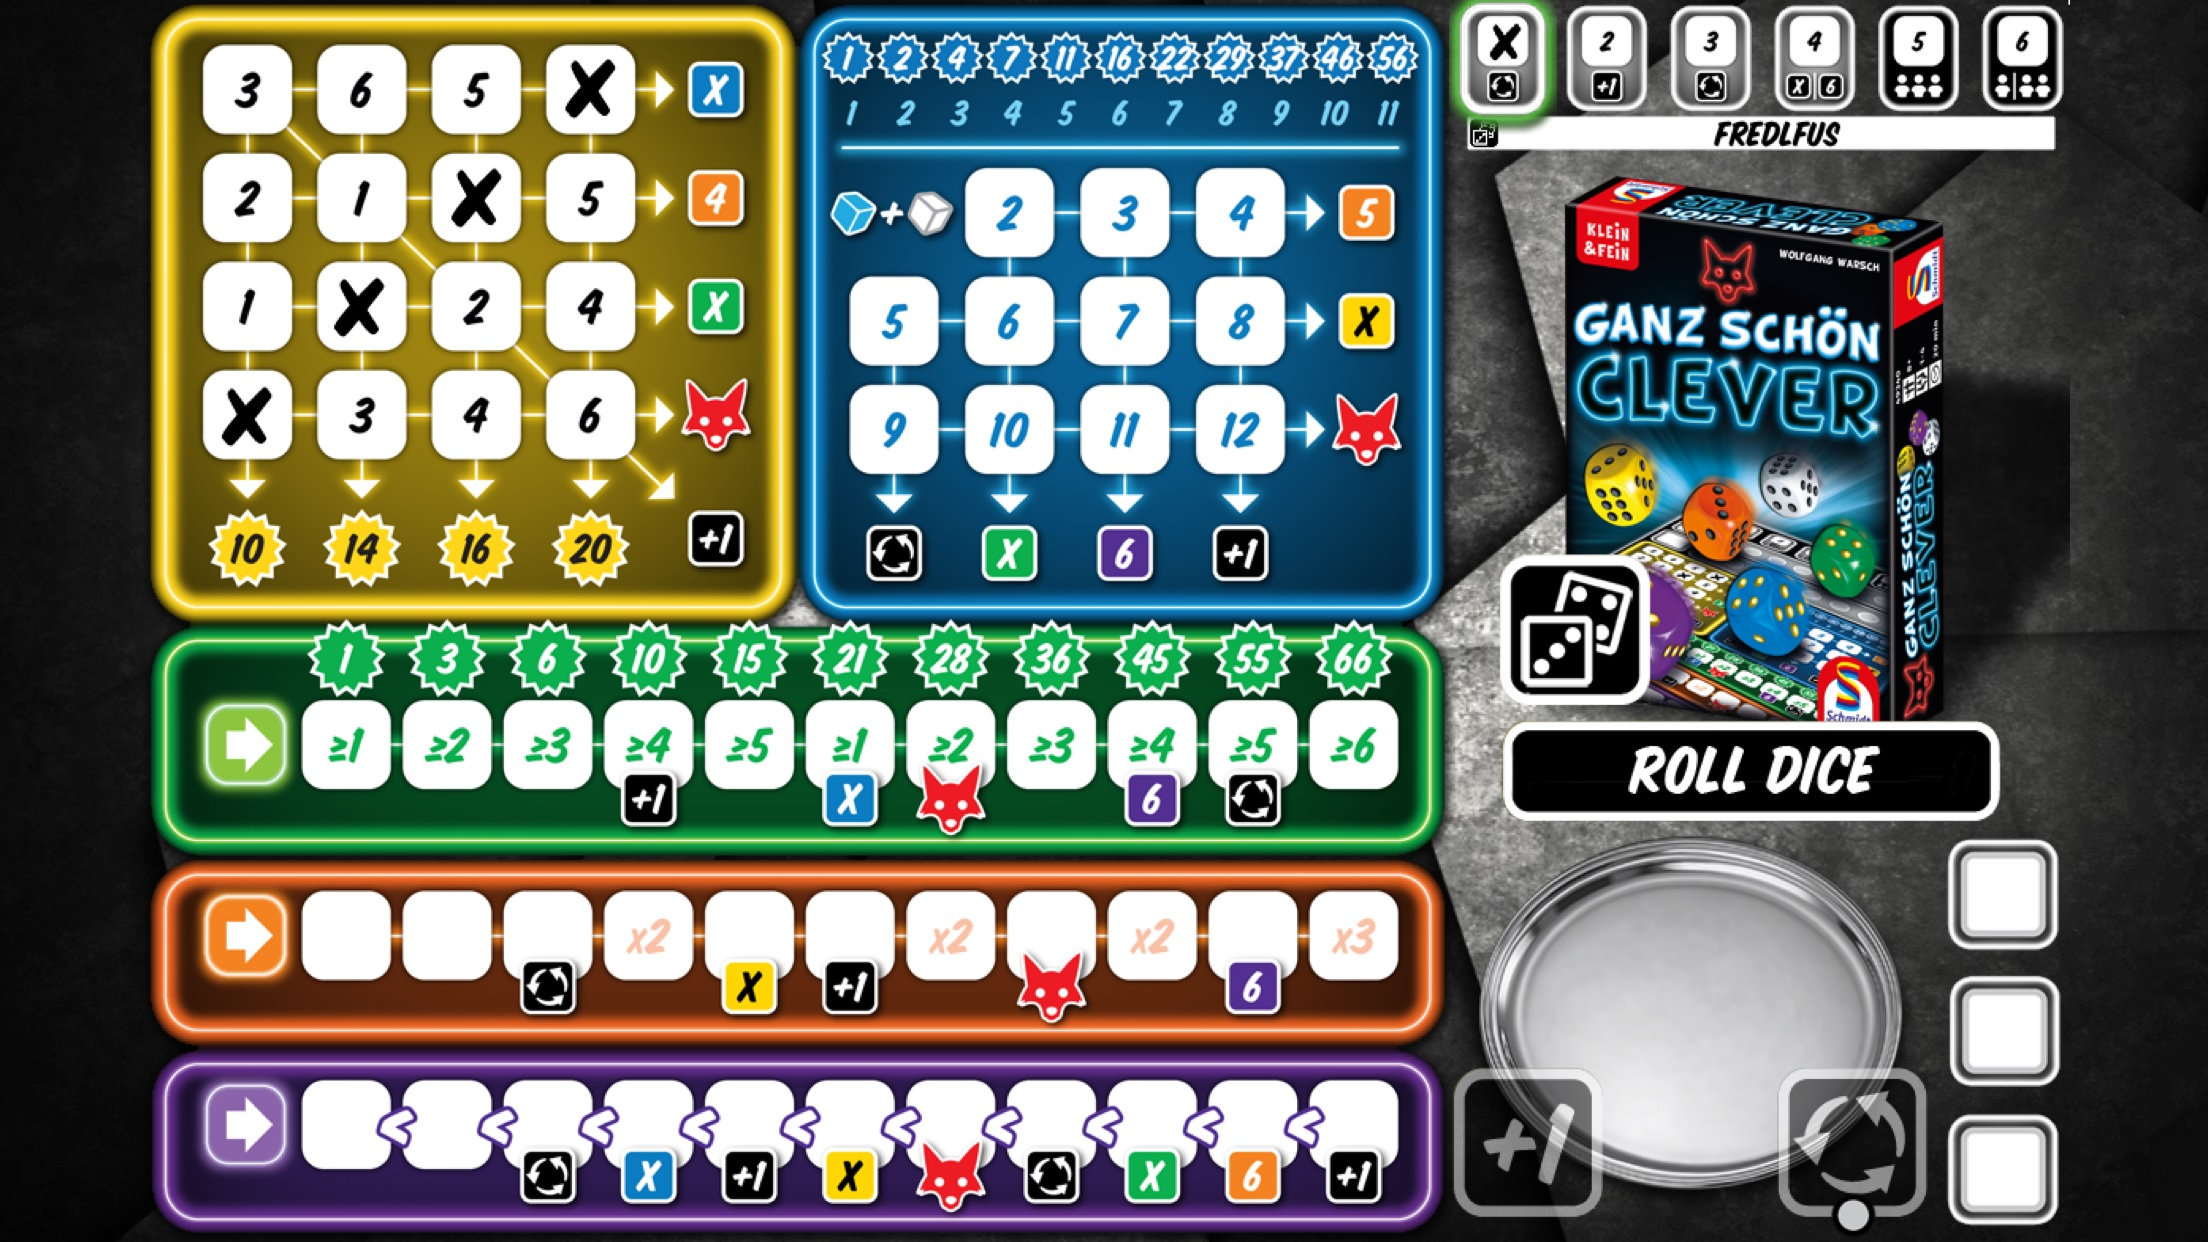
\includegraphics[width=1\textwidth]{Bilder/gsc} 
	\caption[Ganz schön clever]{Ganz schön clever\\ Quelle: Screenshot des Spiels von Brettspielwelt}
\end{figure}

"Ganz schön clever" ist ein Brettspiel, welches von Wolfgang Warsch entworfen und 2018 von Schmidt Spiele veröffentlicht wurde.\\

Im folgenden werden der Spielablauf und die wesentlichen Regeln des Spiels erklärt.

Es gibt sechs farbige Würfel (gelb, blau, grün, orange, lila und weiß), wobei jeder bis auf den weißen einem der 5 farbigen Spielfelder zuzuordnen ist. Der weiße Würfel ist ein Sonderwürfel und kann als einer der anderen Würfel betrachtet werden. Wenn bestimmte Bedingungen erfüllt sind kann der Spieler einen Würfel wählen und das entsprechende Kästchen ausfüllen. Die Felder verfügen über Belohnungen, welche freigeschaltet werden, wenn eine bestimmte Kombination oder Anzahl an Feldern freigeschaltet worden ist. Beim orangenen und lila Feld kommt es bei der Belohnung zudem darauf an wie hoch das Würfelergebnis des gewählten Würfels ist, da die einzelnen Kästchen hier je nach Würfelergebnis zusätzlich belohnt werden.
\\
Das Spiel teilt sich in bis zu sechs Runden mit jeweils bis zu drei Würfen ein. Nach jeder Runde eines Spielers bekommt dieser zudem die Möglichkeit einen Würfel auf dem Silbertablett eines Mitspielers zu wählen. Diese Wahl verhält sich so wie bei der Wahl eines eigenen Würfels bei den Würfen des Spielers selbst. Die Anzahl der Runden werden von der Spielerzahl festgelegt. Bei ein bis zwei Spielern sind es sechs Runden. Bei drei Spielern sind es fünf Runden und bei vier Spielern sind es vier Runden. Die Anzahl der Würfe pro Runde und Spieler ist immer drei, allerdings kann diese Anzahl reduziert werden, wenn kein Würfel mehr zum Würfeln zur Verfügung steht. Dann wird der Spielablauf fortgesetzt als hätte der Spieler seinen dritten Wurf in der Runde beendet und er kann einen Würfel vom Tablett des Mitspielers wählen bevor dann die neue Runde für ihn beginnt. Zu beginn der ersten, zweiten, dritten und vierten Runde bekommt jeder Spieler zudem eine Belohnung, welche oben rechts auf Abbildung 1 bei der jeweiligen Rundenzahl zu sehen ist. Die Belohnung in Runde vier steht dabei für das freie ausfüllen eines beliebigen Kästchens mit dem jeweils maximal möglichen Wert für das Kästchen.

	Die folgende Abbildung zeigt das Runden-System des Spiels. Dieses wird noch einige male wichtig für das Verständnis der Arbeit werden:
	\nopagebreak
\begin{figure}[h]
	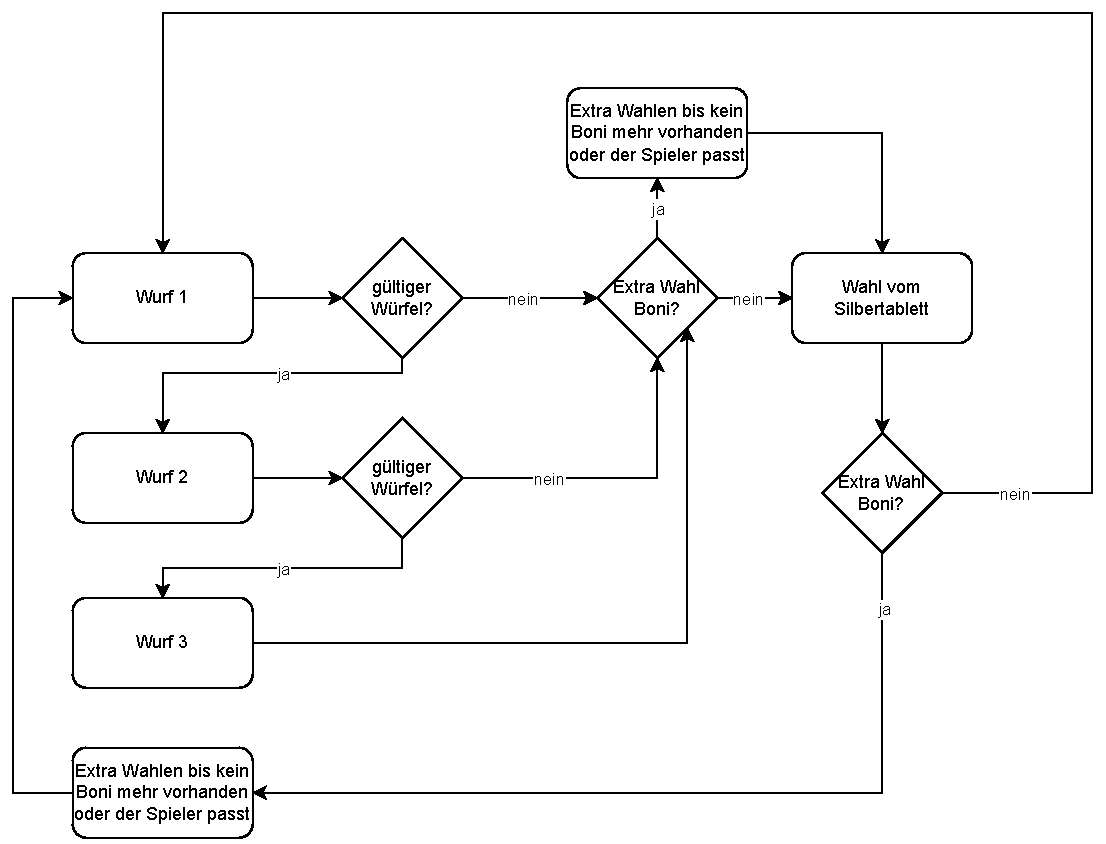
\includegraphics[width=1\textwidth]{Bilder/Rundenablauf.drawio} 
	\caption[Rundenablauf Ganz schön clever]{Rundenablauf Ganz schön clever\\ Quelle: Eigene Darstellung}
\end{figure}

Der Zyklus beginnt bei Wurf 1. Wenn danach noch gültige Würfel vorhanden sind geht es weiter mit Wurf 2. Sind dann noch gültige Würfel vorhanden folgt Wurf 3. Sind in der Zwischenzeit keine gültigen Würfel vorhanden oder spätestens nach Wurf 3 hat der Spieler die Möglichkeit seine Extra Wahl Boni einzusetzen und einen der aktuellen Würfel zu wählen. Entscheidet sich der Spieler dafür keine Extra Wahl Boni einzusetzen oder besitzt er keine, geht es weiter mit der Wahl vom Silbertablett. Dort wählt der Spieler einen Würfel und hat anschließend erneut die Möglichkeit Extra Wahl Boni zu verwenden, falls er mindestens eine besitzt. Entscheidet er sich dafür die Extra Wahl Boni nicht zu benutzen, oder besitzt er keine, beginnt der Zyklus erneut von Wurf 1. Dieser Zyklus wird so lange wiederholt, bis das Spiel endet.\\

Es gibt zwei Arten von Belohnungen im Spiel. Punktebelohnungen und Boni. Bei Punktebelohnungen handelt es sich um Punkte welche auf den Score des Spielers addiert werden, welcher am Ende des Spiels entscheidet wer gewonnen hat. Der Spieler mit dem höchsten Score gewinnt das Spiel. Punktebelohnungen erhält man beim gelben Feld indem man eine Spalte vollständig ausfüllt. Die Anzahl der Punkte findet sich am Ende der Spalte. Im blauen Feld erhält man Punktebelohnungen mit zunehmender Anzahl an ausgefüllten blauen Kästchen. Die Anzahl der Punkte findet sich im oberen Bereich des blauen Feldes. Im grünen Feld ebenso mit zunehmender Anzahl der ausgefüllten grünen Kästchen. Die Anzahl der Punkte findet sich auch hier im oberen Bereich des grünen Feldes. Im orangenen und lila Feld muss man für Punktebelohnungen lediglich ein Kästchen ausfüllen. Die Punktebelohnung entspricht der Augenzahl des entsprechenden ausgefüllten Kästchens. Beim orangenen Feld wird diese Augenzahl bei einigen Feldern zusätzlich mit zwei oder drei multipliziert. Außerdem gibt es eine Boni Belohnung, welche indirekt eine Punktebelohnung darstellt. Es handelt sich hierbei um den sogenannten Fuchs beziehungsweise die Füchse. Die Anzahl der freigeschalteten Füchse wird am Ende des Spiels mit der Anzahl der erzielten Punkte des Feldes mit den niedrigsten erreichten Punktewert multipliziert und zum Gesamtpunktestand addiert.

Bei Boni handelt es sich um Belohnungen, welche der Spieler nutzen kann oder muss, um sich im Spiel einen Vorteil zu verschaffen. Die Boni sind bei den entsprechenden Kästchen beziehungsweise am Rande von Spalten und Zeilen eingezeichnet und können freigeschaltet werden indem man diese (Kästchen beziehungsweise Zeilen oder Spalten) ausfüllt. Eine Ausnahme bildet hier die Boni welche beim gelben Feld freigeschaltet wird indem alle diagonalen Felder von links oben nach rechts unten ausgefüllt werden. \\

Jede Boni hat ihr eigenes Symbol. Nun folgt eine Aufzählung und Erklärung der verschiedenen Boni mit Ausnahme der Füchse. Boni werden bei der Benutzung aufbraucht. Man kann mehr als eine dieser Boni auf einmal besitzen. Die Boni sind stapelbar.

Extra Wahl: Bei der Extra Wahl wird es dem Spieler ermöglicht am Ende seiner eignen Runde beziehungsweise nachdem er einen Würfel vom Silbertablett des Gegners gewählt hat erneut Würfel zu wählen und die entsprechenden Kästchen dafür anzukreuzen. Würfel die so gewählt wurden können mithilfe der Extra Wahl Boni nicht erneut gewählt werden solange keine neue Runde oder Wahl vom Silbertablett beginnt. Mit der Extra Wahl Boni können alle Würfel gewählt werden, nicht nur die, welche unter normalen Umständen gültig zur Wahl stehen würden. Das Symbol ist die +1.

Neuer Wurf: Der Neue Wurf ermöglicht es dem Spieler einen seinen Würfe zu wiederholen ohne dabei einen der Würfel auszuwählen. Dies ermöglicht es ihm Würfe mit ungünstigen Ergebnissen neu auszurichten. Das Symbol sind die drei Pfeile, welche im Kreis angeordnet sind.

Gelbes Kreuz: Ermöglicht es dem Spieler direkt nach erhalten der Boni eines der gelben Kästchen nach eigener Wahl auszufüllen. Das Symbol ist ein Kreuz auf gelbem Hintergrund.

Blaues Kreuz: Ermöglicht es dem Spieler direkt nach erhalten der Boni eines der blauen Kästchen nach eigener Wahl auszufüllen. Das Symbol ist ein Kreuz auf blauem Hintergrund.

Grünes Kreuz: Ermöglicht es dem Spieler direkt nach erhalten der Boni das nächste freie Grüne Kästchen auszufüllen. Das Symbol ist ein Kreuz auf grünem Hintergrund.

Orangene Vier: Ermöglicht es dem Spieler direkt nach erhalten der Boni das nächste freie orangene Kästchen mit einer vier auszufüllen. Das Symbol ist eine vier auf orangenem Hintergrund.

Orangene Fünf: Ermöglicht es dem Spieler direkt nach erhalten der Boni das nächste freie orangene Kästchen mit einer fünf auszufüllen. Das Symbol ist eine fünf auf orangenem Hintergrund.

Orangene Sechs: Ermöglicht es dem Spieler direkt nach erhalten der Boni das nächste freie orangene Kästchen mit einer sechs auszufüllen. Das Symbol ist eine sechs auf orangenem Hintergrund.

Lila Sechs: Ermöglicht es dem Spieler direkt nach erhalten der Boni das nächste freie lila Kästchen mit einer sechs auszufüllen. Das Symbol ist eine sechs auf lila Hintergrund. \\

Nun folgen die Regeln nach denen bestimmt wird ob ein Würfel gewählt werden kann, um ein Kästchen auszufüllen und um zu bestimmen ob er ein gültiger Würfel ist:

Ist ein Würfel ungültig kann dieser nicht gewählt werden. Würfel werden ungültig indem sie in der aktuellen Runde oder bei einer Wahl mit dem Extra Wahl Boni bereits gewählt worden sind. Außerdem werden Würfel, welche eine geringere Augenzahl aufweisen als der aktuell gewählte Würfel automatisch ungültig. Eine Ausnahme ist hierbei die Wahl eines Würfels vom Silbertablett des Gegenspieler oder Wahlen von Würfeln durch die Extra Wahl Boni. Würfel werden wieder gültig am Anfang jeder neuen Runde, nach Abschluss des dritten Wurfes, sowie nach der Wahl des Würfels vom Silbertablett, als auch nachdem Wahlen mit dem Extra Wahl Boni erfolgt sind. Dabei bleiben mithilfe der Extra Wahl Boni gewählte Würfel solange ungültig, bis keine weiteren Extra Wahl Boni in diesem Spielschritt mehr verwendet werden und das Spiel normal weiter geht.

Jedes Feld hat seine eigenen Regeln, die bestimmen, wann ein Kästchen ausgefüllt werden darf. Beim gelben Feld muss die Augenzahl des Würfel mit der Zahl des Kästchens übereinstimmen. Beim Blauen Feld muss die Summe der Augenzahlen des blauen und des weißen Würfels mit der Zahl innerhalb des Kästchens übereinstimmen. Beim grünen Feld muss die Augenzahl des Würfels größer oder gleich der Zahl im Kästchen sein. Zudem kann beim grünen Feld immer nur das nächste freie Kästchen ausgefüllt werden, beginnend von links. Im orangenen Feld kann immer das nächste Kästchen eingetragen werden. Auch hier beginnend von links. Beim lila Feld muss die Augenzahl des Würfels größer sein als die Zahl im zuletzt ausgefüllten Kästchen. Eine Ausnahme bildet hier der Fall in dem eine sechs im zuletzt ausgefüllten Kästchen steht. Dann kann das nächste Feld mit jeder beliebigen Augenzahl gewählt werden. Die sechs setzt die Voraussetzung für das lila Feld bis zum nächsten ausfüllen im lila Feld aus. Auch hier gilt die Reihenfolge von links nach rechts.
\subsubsection{Maschinelles Lernen}
"Maschinelles Lernen heißt, Computer so zu programmieren, dass ein bestimmtes Leistungsmerkmal anhand von Beispieldaten oder Erfahrungswerten optimiert wird" \cite[Seite 3]{alpaydin_maschinelles_2022}.

Es gibt bis heute nach wie vor viele Problemstellungen, die von Menschen auf einfache Art und weise lösbar sind, für die es aber keine algorithmische Lösung zu geben scheint. Hier kommt das maschinelle Lernen zum Einsatz. Durch die Mustererkennung aus Trainingsdaten können Programme lernen solche Problemstellungen zu lösen indem sie präzise Vorhersagen über bestehende Sachverhalte beziehungsweise Muster aus beliebigen Daten des selben oder eines ähnlichen Sachverhaltes, der beim generieren der Trainingsdaten vorhanden war, zu treffen. Ein besonders weit verbreiteter Anwendungsfall ist die Herleitung von Kundenverhalten und möglicher Optimierungsmöglichkeiten für den Verkauf. Wenn man ein Programm verwendet, um eine Struktur mithilfe von maschinellem Lernen zu trainieren, damit diese Vorhersagen über ähnliche Sachverhalte treffen kann, nennt man diese dann Modell. Ein solches Modell wird häufig erst auf allgemeinen Datensätzen und später auf immer spezifischeren Daten trainiert, sodass es schließlich auf eine konkrete Aufgabe zugeschnitten werden kann \cite[Seite 1f]{alpaydin_maschinelles_2022}.

Maschinelles Lernen ermöglicht es zwar nicht einen gesamten Prozess mit all seinen Einzelheiten zu verstehen, aber es ermöglicht relevante Merkmale zu erkennen und mithilfe dieser Merkmale und deren Zusammenhängen Prognosen über einen gesamten Sachverhalt herzuleiten. Auf Grund dieser Prognosen kann schließlich agiert werden. \cite[Seite 2]{alpaydin_maschinelles_2022}.

Die Anwendungsgebiete von maschinellem Lernen sind zahlreich. Unter anderem ist es relevant für den Einzelhandel und Finanzdienstleister, um Kreditgeschäfte abzuwickeln, Betrugsversuche zu erkennen, oder den Aktienmarkt einzuschätzen. Aber auch in der Fertigung wird es zur Optimierung, Steuerung und Fehlerbehebung eingesetzt. Auch in der Medizin erweisen sich medizinische Diagnoseprogramme mithilfe von Modellen, die mit maschinellem Lernen trainiert wurden als nützlich \cite[Seite 3]{alpaydin_maschinelles_2022}.

Die Datenbestände und das World Wide Web werden immer größer und die Suche nach relevanten Daten kann nicht mehr manuell vorgenommen werden. "Das maschinelle Lernen ist aber nicht nur für Datenbanken relevant, sondern auch für das Gebiet der künstlichen Intelligenz" \cite[Seite 3]{alpaydin_maschinelles_2022}. Von Intelligenz spricht man dann, wenn das System selbstständig in einer sich verändernden Umgebung lernen und sich anpassen kann. Dadurch muss der Systementwickler nicht jede erdenkliche Situation vorhersehen und passende Lösungen dafür entwickeln \cite[Seite 3]{alpaydin_maschinelles_2022}.
 
Maschinelles Lernen findet seine Anwendung in dieser Arbeit in Form von Deep Reinforcement Learning. Was Reinforcement Learning ist und wie es sich von Deep Reinforcement Learning unterscheidet wird im Folgenden beschrieben.
\subsubsection{Reinforcement Learning}
Reinforcement Learning (im deutschen: bestärkendes Lernen) heißt so, weil es die Aktionen des Agenten (beziehungsweise des Modells) bestärkt. Man kann sich das in etwa so vorstellen, wie das Training eines Hundes im Park. Dieser wird jedes mal wenn er einen Trick richtig ausführt mit einem Leckerli belohnt. Diese Belohnung bestärkt das Verhalten des Hundes und das Tier lernt dieses in Zukunft zu wiederholen. Eine negative Aktion kann hingegen bestraft werden, damit sie in Zukunft nicht wiederholt wird \cite[Seite 11]{ris-ala_fundamentals_2023}.

Im Reinforcement Learning sind vor allem Folgende Begriffe wichtig:

Agent (oder Modell): Dabei handelt es sich um die Entität, welche mit der Umgebung interagiert und die Entscheidungen trifft. Dabei kann es sich zum Beispiel um einen Roboter oder autonomes Fahrzeug handeln [RL, Seite 11]. In dieser Arbeit ist diese Entität ein Modell, welches mithilfe der Bibliothek Stable-Baselines3 erstellt wird.

Umgebung: Dabei handelt es sich um die Außenwelt des Agenten \cite[Seite 11]{ris-ala_fundamentals_2023}. der Agent interagiert mit dieser und erhält je nach Zustand der Umgebung und seiner gewählten Aktion ein entsprechendes Feedback.

Aktion: Eine Aktion beschreibt das Verhalten des Agenten \cite[Seite 11]{ris-ala_fundamentals_2023}. In dieser Arbeit wählt der Agent Kästchen des Spielbrettes aus, um diese auszufüllen. Außerdem entscheidet er ob er bestimmte Boni zu einem gegebenen Zeitpunkt nutzen möchte oder nicht.

Zustand: Der Zustand beschreibt den Zusammenhang zwischen Umgebung und Agent \cite[Seite 11]{ris-ala_fundamentals_2023}. In dieser Arbeit ist der Zustand von den Eigenschaften des Spielbrettes, der Würfel, der Rundenanzahl und der erspielten Boni abhängig.

Belohnung: Positive oder negative Vergeltung je nachdem wie gut der Zustandswechsel von Zustand x nach Zustand y gewesen ist \cite[Seite 11]{ris-ala_fundamentals_2023}. In dieser Arbeit wird dies durch die jeweiligen Punktebelohnungen im Spiel verkörpert. Eine Ausnahme bildet hier eine negative Belohnung, wenn der Agent in einen Zustand gerät in dem er keine gültige Aktion tätigen kann.

Policy: Die Policy ist die Strategie des Agenten, nach welcher er seine nächsten Aktionen wählt \cite[Seite 11]{ris-ala_fundamentals_2023}. In dieser Arbeit wird die Policy durch ein Multilayer Perceptron (siehe Deep Learning) abgebildet.

Episode: Eine Menge an Zusammenhängenden Aktionen, welche endet, wenn das Ziel erreicht worden ist \cite[Seite 11]{ris-ala_fundamentals_2023}. In dieser Arbeit ist eine Episode ein kompletter Spieldurchlauf von Ganz schön clever.\\

	Die folgende Abbildung beschreibt einen Lernzyklus im Reinforcement Learning:
\nopagebreak
\begin{figure}[h]
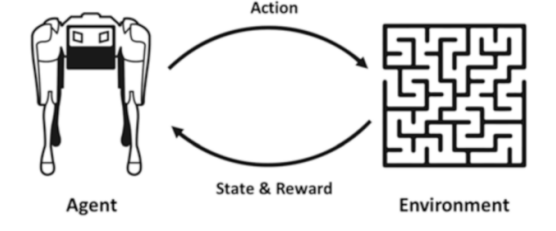
\includegraphics[width=1\textwidth]{Bilder/rl} 
\caption[Reinforcement Learning]{Reinforcement Learning\\ Quelle: \cite{ris-ala_fundamentals_2023}}
\end{figure}

Der Agent führt eine Aktion in der Umgebung aus und erhält daraufhin eine Belohnung und den neuen Zustand der Umgebung als Feedback. Daraufhin aktualisiert er seine Policy, um in Zukunft bessere Aktionen tätigen zu können.

Hierbei ist das Ziel des Agenten die gesamte erreichte Belohnung zu maximieren. Demnach wird die Policy dementsprechend angepasst, dass dies begünstigt wird \cite[Seite 12f]{ris-ala_fundamentals_2023}.

Doch dabei gibt es einige Schwierigkeiten, die es zu beachten gilt. Belohnungen die in kurzer Zeit erreicht werden können, könnten wichtiger oder weniger wichtig sein als Belohnungen, die erst innerhalb vieler Schritte erreicht werden können. Ein gutes Beispiel hierfür wäre ein Balanceakt, bei dem es besonders wichtig ist kurzzeitige Belohnungen zu bevorzugen, da die Episode endet, wenn das Balancieren fehlschlägt, was eine starke negative Belohnung zur Folge haben kann.

Ein weiterer Faktor ist die Balance zwischen Erkundung und Ausbeutung. Diese zwei Prinzipien sind wesentlich für das Reinforcement Learning. Dabei geht es darum, wie stark die Policy es vorzieht neue oder selten gesehene Zustände und Aktionen auszuprobieren oder bereits bekannte, welche eine gute Belohnung zu bringen scheinen auszunutzen beziehungsweise auszubeuten \cite[Seite 13]{ris-ala_fundamentals_2023}.

Im Grunde lernt das Modell, in bestimmten Zuständen bestimmte Aktionen zu tätigen, um das beste Gesamtergebnis zu erreichen. Jeder Zustand hat seinen erwarteten Wert beziehungsweise seine erwartete Belohnung, sobald das Modell in einen bestimmten Zustand gerät, wählt es die Aktion, welche die höchste erwartete Belohnung bietet beziehungsweise weist den möglichen Aktionen Wahrscheinlichkeiten zu, die bei bevorzugten Aktionen höher ausfallen.\\

Die folgende Abbildung zeigt einen Ausschnitt eines theoretischen Zustandsverlaufs von zwei Würfen des Spiels Ganz schön clever:
\nopagebreak
\begin{figure}[h]
	\includegraphics[width=1\textwidth]{Bilder/Baumdiagramm_Spielzustände.drawio} 
	\caption[Zustandsverlauf Ganz schön clever]{Zustandsverlauf Ganz schön clever\\ Quelle: Eigene Darstellung}
\end{figure}	

Das Spiel beginnt. Die Würfel werden gewürfelt und der Agent wählt einen der sechs Würfel mit einer bestimmten Augenzahl und füllt das entsprechende Kästchen aus. Somit gerät er in einen neuen Zustand bei dem ein bestimmtes Kästchen ausgefüllt und ein oder mehrere Würfel ungültig sind. Die gültigen Würfel werden erneut geworfen und er wählt erneut einen der Würfel mit einer bestimmten Augenzahl und füllt das entsprechende Kästchen aus. Es ist schnell zu erkennen, dass sich eine große Zahl an möglichen Zustands-Aktions-Paaren ergibt. Ein Zustands-Aktions-Paar beschreibt genau eine mögliche Aktion in einem spezifischen Zustand des Spiels. Das Modell lernt durch die Auswertung eben dieser Zustands-Aktions-Paare, welche Aktionen am vorteilhaftesten sind und welche er vermeiden sollte. Die Abbildung ist lediglich eine Vereinfachung, da viele weitere Faktoren, wie erspielte Boni eine Rolle spielen.
\subsubsection{Deep Learning}
Von Deep Learning spricht man sobald ein Neuronales Netz mehrere versteckten Schichten hat. 

Ein solches Netz besteht aus einer Vielzahl von Neuronen \cite[Seite 75]{sewak_deep_2019}. Ein solches Neuron setzt sich zusammen aus Inputs, Outputs, Gewichtungen dieser In- und Outputs, sowie einer Aktivierungsfunktion, welche auch gewichtet sein kann. Ein Spezialfall eines solchen Neuronalen Netzes ist ein sogenanntes Multilayer Perceptron. Bei diesem sind alle Neuronen in einer Schicht mit allen Neuronen der folgenden Schicht verbunden. Häufig haben auch alle Neuronen der versteckten Schichten die selbe Aktivierungsfunktion. Was den Beitrag der einzelnen Neuronen zum Gesamtergebnis des Netzes steuert sind im wesentlichen seine Gewichtungen und die Position im Netz.\\

Die folgende Abbildung zeigt ein solches Multilayer Perceptron:
\nopagebreak
\begin{figure}[H]
	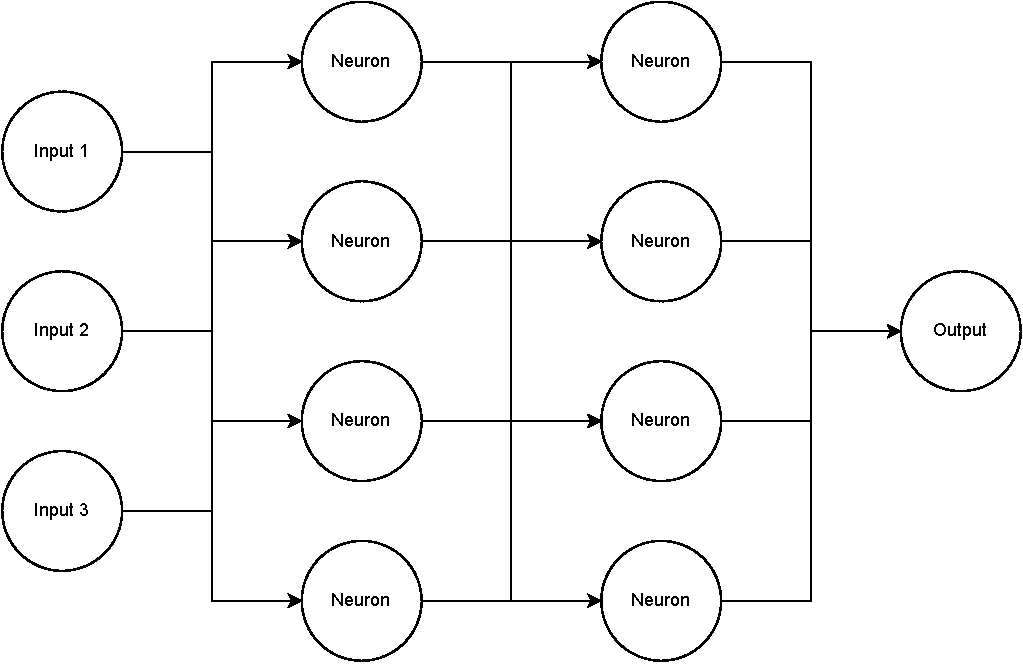
\includegraphics[width=1\textwidth]{Bilder/mlp2.drawio} 
	\caption[Multilayer Perceptron]{Multilayer Perceptron}
\end{figure}	

Die Inputs des Netzes sind die Werte von Variablen der zur Verfügung stehenden Beobachtungen der Umgebung. Die versteckten Schichten verarbeiten diese Inputs dann mit ihren Funktionen und Gewichtungen. Das Output des Netzes ist hingehen eine gewünschte Vorhersage, die mit ihrer eigenen Aktivierungsfunktion hergeleitet wird.
\subsubsection{Proximal Policy Optimization}
Proximal Policy Optimization oder kurz PPO ist eine neue Policy Gradient Methode für Reinforcement Learning. Im Gegensatz zu standardmäßigen Policy Gradient Methoden ist es mit dieser Methode möglich mehrere Policy Updates pro Datenpaket durchzuführen. PPO hat einige der Vorteile der Trusted Region Policy Optimization (kurz TRPO), ist aber simpler zu implementieren und hat auch andere Vorteile, wie bessere Generalisierbarkeit und niedrigere Stichprobenkomplexität. PPO zeigt eine gute Balance zwischen Stichprobenkomplexität, Einfachheit und Trainingsgeschwindigkeit \cite[Seite 1]{schulman_proximal_2017}.

Die Stichprobenkomplexität beschreibt wie groß ein Datenpaket sein muss, um dem Algorithmus ein gewisses Level an Performanz zu ermöglichen. Dies ermöglicht es mehr Updates mit weniger Gesamtdaten durchzuführen, was vor allem hilfreich ist, wenn nicht genügend Daten zur Verfügung stehen oder diese nur schwer zu generieren sind.

Policy Gradient Methoden berechnen einen Gradienten und passen die Policy in Richtung der negativen Steigung an. Das kann man sich ähnlich wie einen Punkt auf einer Parabel vorstellen, die Policy entspricht dem Punkt und wird so lange angepasst beziehungsweise verschoben, bis sie möglichst das Minimum der Parabel erreicht. Dieses Minimum spiegelt eine optimale Policy wieder.

Bei der Trusted Region Policy Optimization gibt es eine vertrauenswürdige Region innerhalb derer die Policy abgeändert werden darf. Das soll sicherstellen, dass die Policy nicht zu stark abgeändert wird, um ein stabileres Training zu gewährleisten. Im Gegensatz zur PPO werden Änderungen, die zu stark abweichen verworfen.

Bei der PPO kommt es zum sogenannten Clipping. Hierbei werden zu starke Änderungen im übertragenen Sinne abgeschnitten und es kommt zu einer abgeschwächten Änderung der Policy.

PPO ist ein verhältnismäßig simpler, einfach zu verstehender und dennoch effizienter Algorithmus. Er hat eine gute Balance zwischen Stabilität und Effizienz. Außerdem erzielt er gute Ergebnisse bei einer großen Bandbreite an Aufgaben \cite{schulman_proximal_2017}. Daher eignet sich PPO besonders gut für Einsteiger, die bisher nicht viel mit Deep Reinforcement Learning gearbeitet haben.
\subsection{Verwendete Technologien}
\subsubsection{Gymnasium}
Gymnasium ist die Fortführung der OpenAi Bibliothek Gym \cite{noauthor_gymnasium_nodate}. Sie kann genutzt werden, um Umgebungen zu schaffen, die für maschinelles Lernen verwendet werden können. Die Bibliothek bietet auch eine Menge vordefinierter Umgebungen, welche kostenfrei genutzt werden können, was gerade für Einsteiger den Vorteil hat sich mit wenig Aufwand ausprobieren zu können.

Die Bibliothek bietet Kernmethoden, welche später selbst gefüllt und implementiert werden müssen, um die Bibliothek mit einer benutzerdefinierten Umgebung nutzen zu können. Die wesentlichen Methoden, welche auf jeden Fall implementiert werden müssen sind die Schritt-Methode (im Englischen step-method) und eine Methode zum zurücksetzen der Umgebung auf den Startzustand (im Englischen reset-method). Außerdem muss eine Initialisierung der Umgebungsklasse erfolgen. Die Schritt-Methode nimmt eine Aktion entgegen und führt diese in der Umgebung aus. Außerdem liefert sie den Zustand der Umgebung nach dem Ausführen der Aktion und die Belohnung für den ausgeführten Schritt zurück. Die Reset-Methode setzt alle relevante Werte der Umgebung auf den Ausgangswert zurück, sodass das Spiel oder die Aufgabe von vorne gestartet werden kann. Des Weiteren bietet es sich an eine Methode zu implementieren, welche den aktuellen Zustand der Umgebung zurückgibt, dies ist allerdings optional.

Gymnasium bietet eine gute Anbindung an die Bibliothek Stable Baselines 3, welche Methoden zum Trainieren eines Modells auf Basis einer eben solchen Gymnasium Umgebung bietet. In dieser Arbeit wird Gymnasium für die Implementierung der Spielumgebung von Ganz schön clever verwendet, damit diese anschließend mithilfe von Stable Baselines 3 trainiert werden kann.
\subsubsection{Stable Baselines 3}
"Stable Baselines 3 ist eine Bibliothek, welche verlässliche Implementierungen von Reinforcement Learning Algorithmen in Pytorch bietet" \cite[Seite 1]{noauthor_stable-baselines3_nodate}. 

Die Algorithmen haben ein konsistentes Interface und eine umfangreiche Dokumentation, was es einfach macht verschiedene Reinforcement Learning Algorithmen zu testen. Die Implementierung bietet eine simple API. Modelle können in nur wenigen Codezeilen trainiert werden. Die Implementierung weist zudem eine hohe Qualität auf. Es gibt auch eine experimentelle Version der Bibliothek, welche Stable Baseline 3 Contributing genannt wird \cite[Seite 1-3]{noauthor_stable-baselines3_nodate}.

In diese Arbeit wird vor Allem der MaskablePPO Algorithmus aus eben dieser Contributing Bibliothek benutzt. Dabei handelt es sich, um eine Erweiterung des PPO Algorithmus von Stable Baseline 3. Dieser MaskablePPO erweitert den PPO Algorithmus um die Funktionalität einer Maskierung. Diese Maskierung ermöglicht es die Wahlwahrscheinlichkeit bestimmter Aktionen auf Null zu setzen. Die Maskierung wurde in der Arbeit verwendet, um ungültige Aktionen auszuschließen, sodass das Modell nicht auf andere Weise lernen muss, diese zu vermeiden. Dies ist ein simpler und effizienter Weg, um zu gewährleisten, dass beim Training keine ungültigen Aktionen gewählt werden.
\subsubsection{Matplotlib}
Matplotlib ist eine umfangreiche und mächtige Bibliothek zum Plotten von Daten. In dieser Arbeit wird Matplotlib dafür verwendet, um die erreichten Punkte und ungültigen Züge zu visualisieren.
\subsubsection{ChatGPT 4}
ChatGPT 4 ist die neueste Version eines neuartigen Chat-Bots. Dieser ermöglicht es dem Benutzer Fragen zu stellen oder aussagen zu treffen, auf die er dann eine Antwort bekommt. Die Erzeugnisse des Chat-Bots sind so gut, dass er sich gut eignet, um bei der Konzeption und Programmierung der Arbeit zu unterstützen. Daher wird ChatGPT 4 in dieser Arbeit zum Teil als Hilfestellung bei Unklarheiten zur Funktionsweise von Technologien und beim Bau des Prototypen verwendet. 

Zudem wird im Rahmen der Arbeit analysiert wie gut sich ChatGPT 4 als unterstützendes Werkzeug eignet und welche Vor- und Nachteile, sowie welche Einschränkungen die Nutzung mit sich bringt.